\begin{figure}[ht]
  \centering
  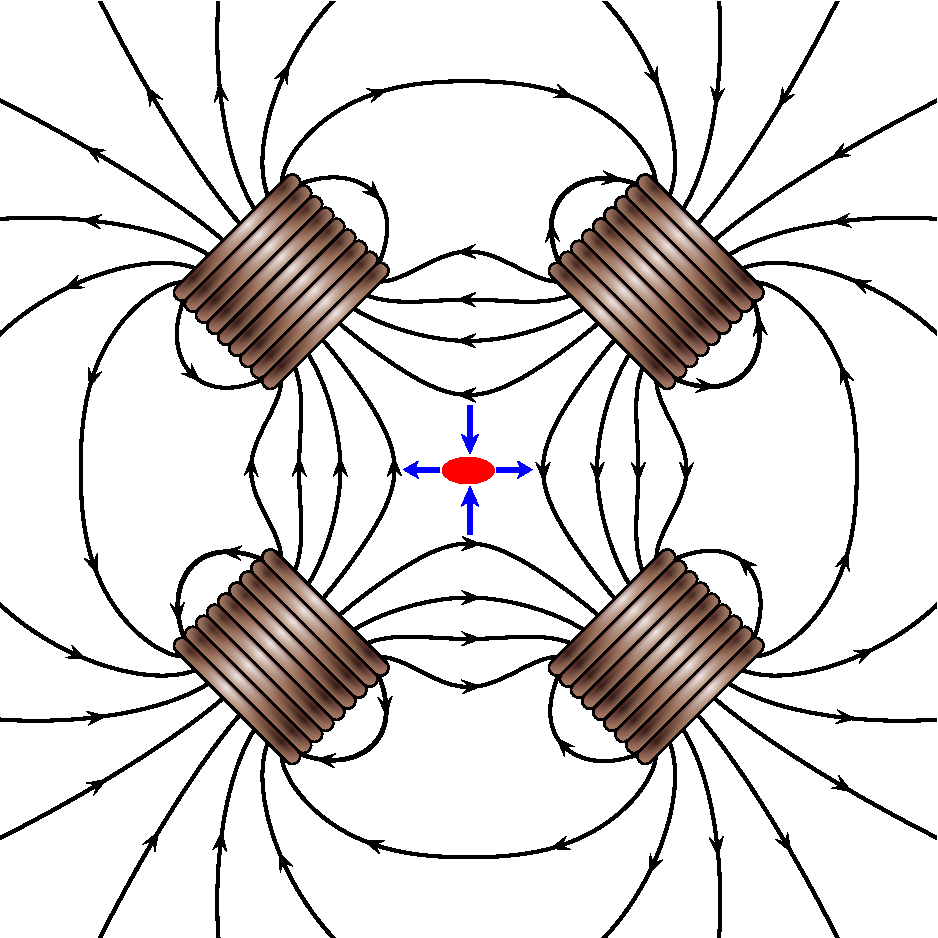
\includegraphics[trim={0 0.7cm 0 0.5cm}, clip,
  width=.6\textwidth]{quarupole_with_beamspot}
  \caption{Representation of an idealised set of coil magnets in a quadrupole
    configuration with a proton beamspot shown as a red ellipse. The proton beam
    is drawn coming out of the page (\emph{watch out!}), magnetic field lines
    are drawn in black and the forces acting on each bunch of protons are drawn
    as blue arrows.}
  \label{fig:quadrupole}
\end{figure}
